\documentclass[11pt]{article} 
\usepackage[utf8]{inputenc}

%%% PAGE DIMENSIONS
\usepackage{geometry}
\geometry{a4paper}

\usepackage{graphicx} % support the \includegraphics command and options

% \usepackage[parfill]{parskip} % Activate to begin paragraphs with an empty line rather than an indent

%%% PACKAGES
\usepackage{float}
\usepackage{booktabs}
\usepackage{array}
\usepackage{paralist}
\usepackage{verbatim}
\usepackage{subfig} 
\usepackage{fancyhdr}


\pagestyle{fancy} % options: empty , plain , fancy
\renewcommand{\headrulewidth}{0pt} % customise the layout...
\lhead{}\chead{}\rhead{}
\lfoot{}\cfoot{\thepage}\rfoot{}

\usepackage{sectsty}
\allsectionsfont{\sffamily\mdseries\upshape}

\usepackage{listings}
\usepackage{color}

\definecolor{mygreen}{rgb}{0,0.6,0}
\definecolor{mygray}{rgb}{0.5,0.5,0.5}
\definecolor{mymauve}{rgb}{0.58,0,0.82}

\lstset{ 
  backgroundcolor=\color{white},   % choose the background color; you must add \usepackage{color} or \usepackage{xcolor}; should come as last argument
  basicstyle=\footnotesize,        % the size of the fonts that are used for the code
  breakatwhitespace=false,         % sets if automatic breaks should only happen at whitespace
  breaklines=true,                 % sets automatic line breaking
  captionpos=b,                    % sets the caption-position to bottom
  commentstyle=\color{mygreen},    % comment style
  firstnumber=1000,                % start line enumeration with line 1000
  frame=single,	                   % adds a frame around the code
  keepspaces=true,                 % keeps spaces in text, useful for keeping indentation of code (possibly needs columns=flexible)
  keywordstyle=\color{blue},       % keyword style
  language=Python,                 % the language of the code
  numbers=left,                    % where to put the line-numbers; possible values are (none, left, right)
  numbersep=5pt,                   % how far the line-numbers are from the code
  numberstyle=\tiny\color{mygray}, % the style that is used for the line-numbers
  rulecolor=\color{black},         % if not set, the frame-color may be changed on line-breaks within not-black text (e.g. comments (green here))
  showspaces=false,                % show spaces everywhere adding particular underscores; it overrides 'showstringspaces'
  showstringspaces=false,          % underline spaces within strings only
  showtabs=true,                   % show tabs within strings adding particular underscores
  stepnumber=1,                    % the step between two line-numbers. If it's 1, each line will be numbered
  stringstyle=\color{mymauve},     % string literal style
  tabsize=2,	                   % sets default tabsize to 2 spaces
  title=\lstname                   % show the filename of files included with \lstinputlisting; also try caption instead of title
}


\title{Práctica 1: Regresión Lineal}
\author{Ana Martín Sánchez, Nicolás Pastore Burgos}
\date{21/09/2021} 

\begin{document}
\maketitle

\section{Descripción de la práctica}

 En esta práctica, se pedía aplicar el método de regresión lineal sobre dos conjuntos de datos. 
 
 En primer lugar, se nos da un conjunto de datos que relaciona dos variables: la población de una ciudad con los beneficios de una compañía de distribución de comida en dicha ciudad.
 Después, se nos presenta un conjunto de datos que relaciona el precio de casas vendidas en Portland con el tamaño en pies cuadrados, el número de habitaciones y el precio de dicha casa.

 Para el primer conjunto de datos, se puede aplicar el método de regresión lineal con una variable; es evidente que, en el segundo caso, no es así.

 Para agilizar esta segunda parte, es necesario normalizar los atributos, antes de aplicar un descenso de gradiente.

 Por último, aplicaremos el método de la ecuación normal sobre el segundo conjunto de datos, con el fin de comprobar que nuestros cálculos anteriores son correctos.


\newpage
\section{Solución propuesta}

\subsection{Resultados obtenidos}

\subsubsection {Parte 1}

En esta parte hemos conseguido los reultados esperados; hemos podido implementar una función de descenso de gradiente que es capaz, dados unos datos, de calcular una ecuación lineal que minimice los costes. Para comprobarlo, hemos utilizado el ejemplo propuesto en el enunciado (para una población de 70.000 habitantes, los beneficios estimados son de 45.282\$). 

 \begin{figure}[h!]
    \begin{center}
    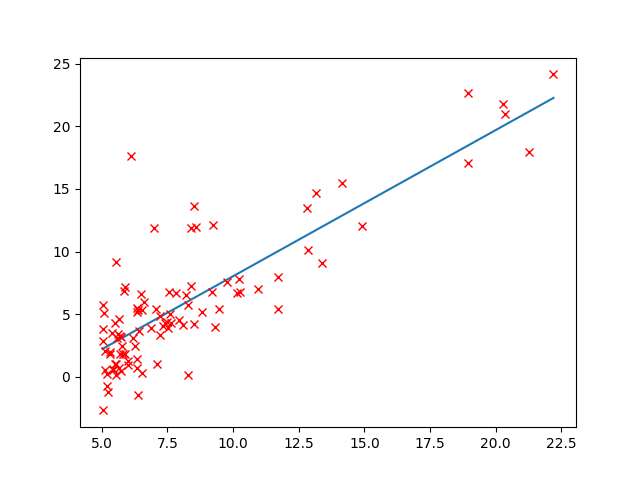
\includegraphics[width=\textwidth]{Imagenes/gradiantDescenseResult.png}
    \caption{Gráfica que muestra la recta calculada para los datos proporcionados por el enunciado.}
    \label{fig:Gráfica que muestra la recta calculada para los datos proporcionados por el enunciado.}
    \end{center}
 \end{figure}
Además, hemos generado las gráficas que muestran los costes, como se muestran a continuación.

 \begin{figure}[h!]
    \begin{center}
    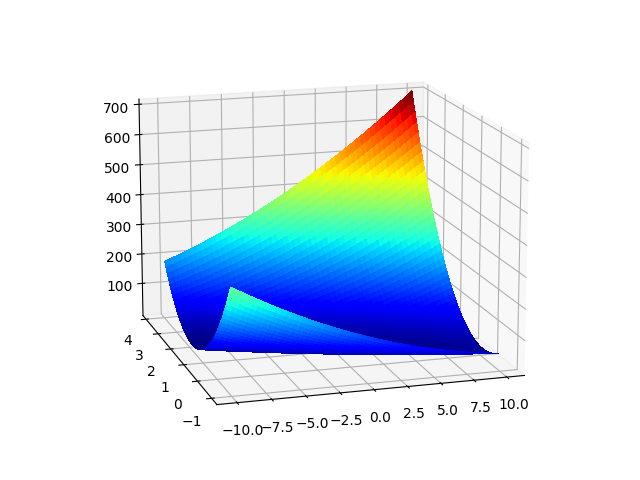
\includegraphics[width=0.45\textwidth]{Imagenes/costMap.png}
    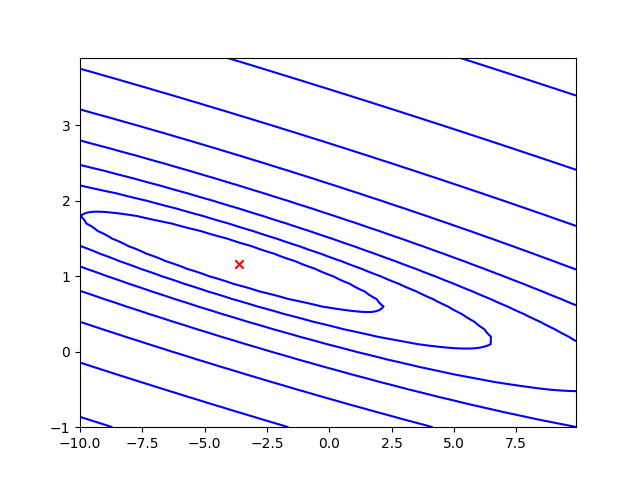
\includegraphics[width=0.45\textwidth]{Imagenes/costMap2.png}
    \caption{Representación de una sección de la ecuación que siguen las thetas.}
    \label{fig:Representación de una sección de la ecuación que siguen las thetas.}
    \end{center}
 \end{figure}

\subsubsection {Parte 2}

En esta segunda parte, también hemos implementado un descenso de gradiente, pero con un número n de atributos. Además hemos implementado la ecuacuón normal.

Para comprobar que ambas implementaciones eran correctas, hemos utilizado el ejemplo propuesto en el enunciado (la entrada [1650, 3]), y ambas nos daban el mismo resultado (293098.46), con una diferencia de menos del 0.01\% entre ambos resultados.

Como comprobación adicional, hemos observado que la función de costes devuelve un resultado cada vez menor, como se puede observar a continuación.

 \begin{figure}[h!]
    \begin{center}
    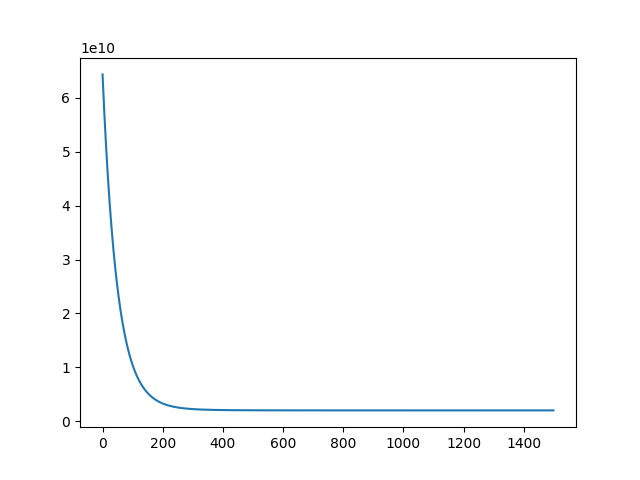
\includegraphics[width=0.6\textwidth]{Imagenes/gradiantDescenseResult2.png}
    \caption{La función de costes es cada vez menor.}
    \label{fig:Resultados}
    \end{center}
 \end{figure}

\newpage
\subsection{Implementación}

\lstinputlisting[language=Python]{main.py}


\end{document}
